%% V1.0
%% by Gabriel Garcia, gabrcg@gmail.com
%% This is a template for Udacity projects using IEEEtran.cls

%% Be Udacious!

\documentclass[10pt,journal,compsoc]{IEEEtran}

\usepackage[pdftex]{graphicx}    
\usepackage{cite}
\usepackage{listings}
\hyphenation{op-tical net-works semi-conduc-tor}

\lstset{
 columns=fixed,       
 numbers=left,                                           
 language=c++,                                   
}

\begin{document}

\title{Localization Project - Where Am I}

\author{Hanwei Zhang(WSYiDao)}

\markboth{Robotics Nanodegree Program Homework}%
{}
\IEEEtitleabstractindextext{%

\begin{abstract}
Project required develop a mobile robot model for Gazebo, and integrate the AMCL(Adaptive Monte Carlo Localization) and Navigation ROS packages for localizing the robot in the provided map. In order to reach the goal successful, it need to add and tune parameters for the running ROS packages to improve the test localization results.Two different robot models are considered for performance evaluation. After achieving the desired results for the robot model introduced in the lesson, a new robot model was made with significant changes , by tuning parameters it reach the goal successfully.
\end{abstract}

% Note that keywords are not normally used for peerreview papers.
\begin{IEEEkeywords}
Robotics, Gazebo, AMCL, Udacity, Localization.
\end{IEEEkeywords}}


\maketitle
\IEEEdisplaynontitleabstractindextext
\IEEEpeerreviewmaketitle
\section{Introduction}
\label{sec:introduction}

\IEEEPARstart{L}ocalization is the challenge of determining the robot's position in a mapped environment, by implementing a probabilistic algorithm to filter noisy sensor measurements and track the robot's position and orientation. In the project, we simulate a robot in real world with a known map to approximate the current position and move to the goal position, by using the localization algorithm and the ROS packages.



\section{Background}
Extended Kalman Fitel(EKF) and Monte Carlo Localization(MCL) are two popular localization algorithms. EKF is the most common Gaussian filter that helps in estimating the state of non-linear models, and MCL is a particle filter because is estimates the robot's pose using particles.In the real world, the environment which is dynamic where objects may shift over time,  and static environments where it always matches the ground truth map. They all faced noisy sensor measurements and it's important to estimate the current pose of the robot with a acceptable computational complexity.

\subsection{Kalman Filters}
Kalman Filters is a very robust algorithm for filtering noisy sensor data. Unlike other algorithms that require a lot of data to make an estimate, the Kalman Filters is able to do so after juct a few sensor maesurements. It does so by using an initial guess and by taking into account the expected uncertainty of a sensor or movement. Sensor fusion is also a good way to localization by  using the Kalman filter to calculate a more accurate estimate location using data from multiple sensors. 

\subsection{Particle Filters}
Each particles represents the hypothesis of there the robot might be. They are each assigned a weight, the weight of the particles is the difference between the actual pose and the predicted pose. The importance and accurate of a particle depends on its weight, and the large weights particles are more likely to survive after a resampling process. Particle Filters will converge and estimate the robot's pose after several iterations and different stages of resampling.

\subsection{Comparison / Contrast}
Compare to the MCL, the Kalman Filters is often used to a Linear Gaussian state space assumption that can only solve the position tracking problem. Kalman Filter and EKF is a good algorithm in a sensor fusion system by estimate different maturement togather and in a fast motion and estimation system with small cost of compute resources. MCL can be applied to more systems with nonlinear and global lacalization, and by tuning parameters it can control the computation memory and resolution. In the model state space, MCl use muti-model discrete  and EKF is unimodal Continuous.


\section{Simulations}
In the robot simulation,  robot model designed by using Universal Robotic Description Format(URDF), include two wheels on the left and right side of the chassis, two wheels front and back below the chassis, cameras in front of the box and a Hokuyo laser on the front top of the box. In the project, I use ROS AMCL package, Move Base package and modified ROS packages udacity\_bot for first robot test. The second develop robot in files develop\_config and urdf\_develop ,if substitute files config and urdf could run the develop robot test.

\subsection{Achievements}
The benchmark model and the own developed model both reach the goal state and passed the navigation\_goal.cpp test.

% Robot Models
\subsection{Benchmark Model}
see Fig. \ref{fig:Benchmark}

\begin{figure}
\centering
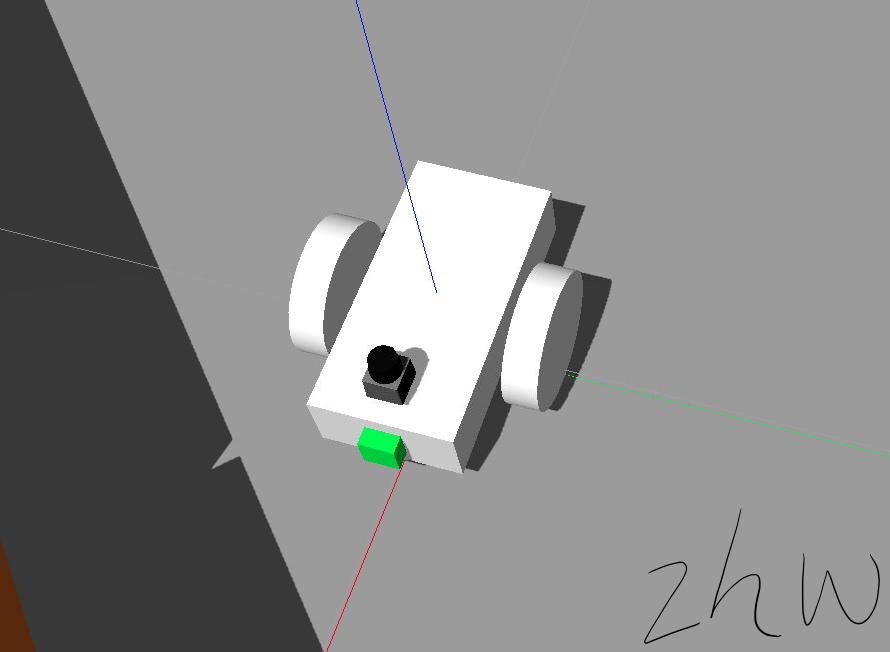
\includegraphics[width=0.5\textwidth]{r8.png}
\caption{\label{fig:Benchmark}Result 2:Develop robot has reached the goal position and pass the test.}
\end{figure}

\subsubsection{Model design}
In the benchmark model, chassis with the size of (.4 .2 .1), two cylinder wheels on the left and right side of the chassis with the size of radius "0.1" and length '0.05', two sphere wheel on the front and back size below the chassis.


\subsubsection{Packages Used}
In the project ,ROS AMCL package and Move Base package are used to localize the position and navigate the robot to the goal position.

\subsubsection{Parameters}


\begin{lstlisting}
"base_local_planner_params.yaml"
TrajectoryPlannerROS:
  holonomic_robot: false
  yaw_goal_tolerance: 0.1
  xy_goal_tolerance: 0.1
  sim_time: 1.0
  meter_scoring: true 
  controller_frequency: 15.0
\end{lstlisting}


\begin{lstlisting}
"costmap_common_params.yaml"
  map_type: costmap
  obstacle_range: 3.0
  raytrace_range: 5.0
  transform_tolerance: 0.3
  inflation_radius: 0.3
  observation_sources: laser_scan_sensor
  laser_scan_sensor: {sensor_frame: hokuyo, 
  data_type: LaserScan, 
  topic: /udacity_bot/laser/scan, 
  marking: true, clearing: true}
\end{lstlisting}


\subsection{Personal Model}

\begin{figure}
\centering
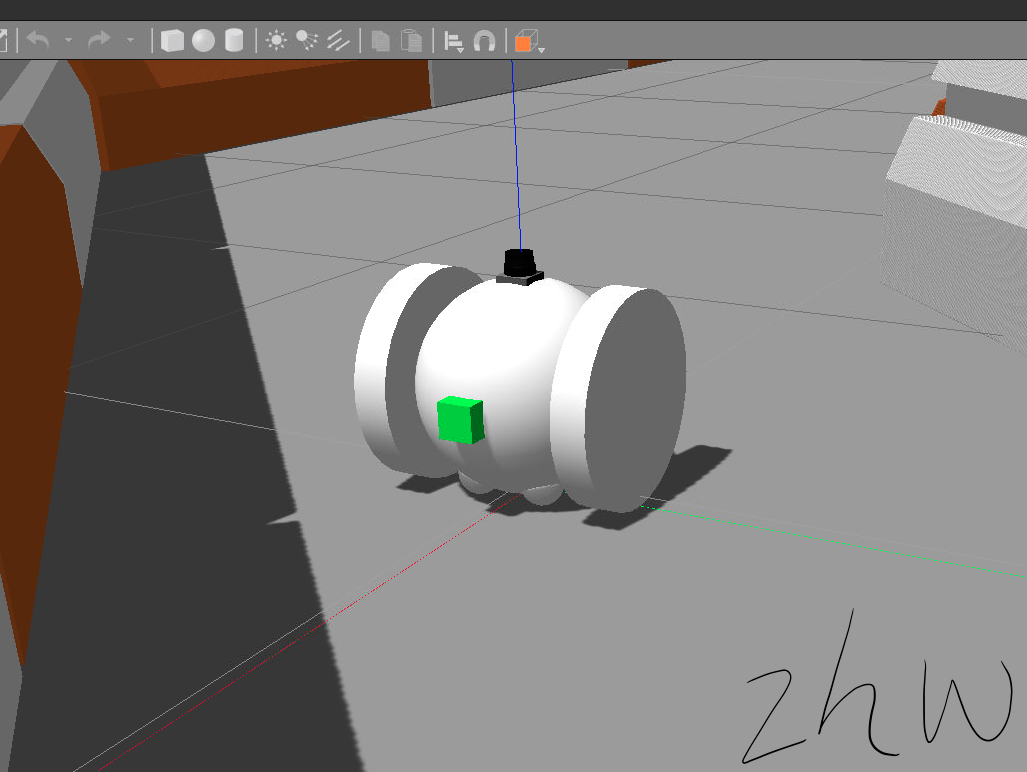
\includegraphics[width=0.5\textwidth]{r6.png}
\caption{\label{fig:frog}Personal model 1.}
\end{figure}

\begin{figure}
\centering
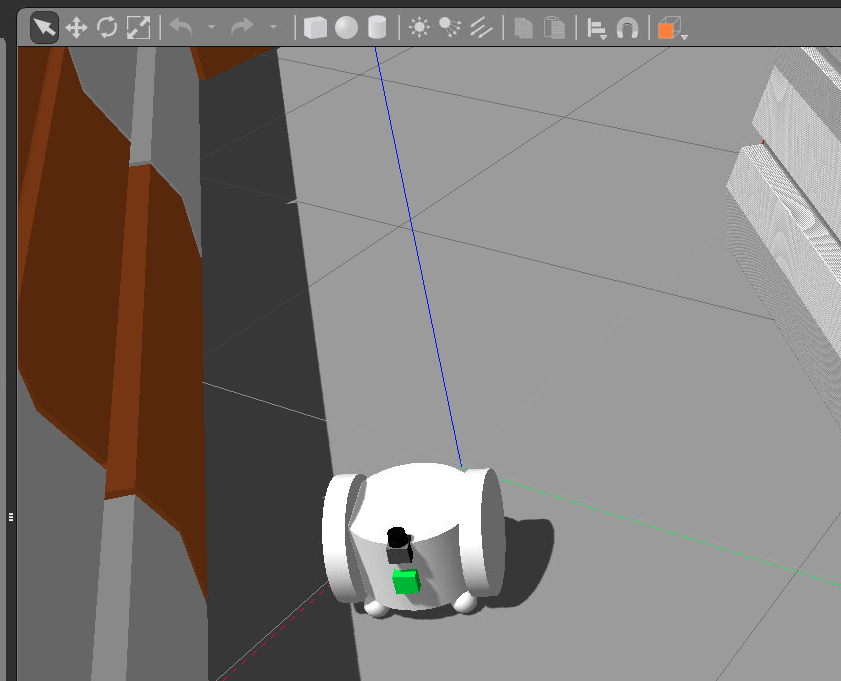
\includegraphics[width=0.5\textwidth]{r10.png}
\caption{\label{fig:frog}Personal model 2.}
\end{figure}

\begin{figure}
\centering
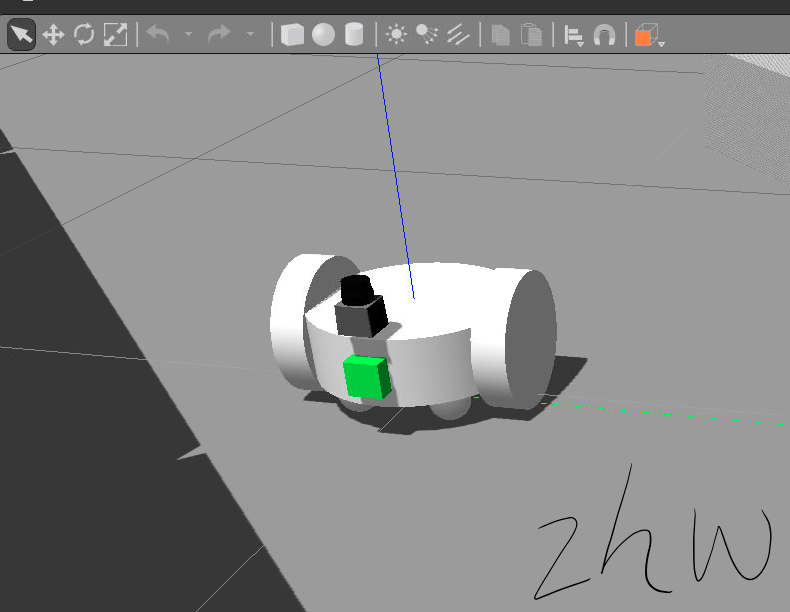
\includegraphics[width=0.5\textwidth]{r13.png}
\caption{\label{fig:frog}Personal model 3.}
\end{figure}

\subsubsection{Model design}
In the develop model, I try three kinds of model and find a best one (Personal model 3).
The best personal model Robot included: chassis with the cylinder size of length "0.1" radius"0.15", four sphere wheel below the chassis size of  radius"0.0299", two cylinder wheels on the left and right side of the chassis with the size of radius "0.1" and length '0.05', 
\subsubsection{Packages Used}
In this part, ROS AMCL package and Move Base package are used to localize the position and navigate the robot to the goal position.

\subsubsection{Parameters}


\begin{lstlisting}
"base_local_planner_params.yaml"
TrajectoryPlannerROS:
  holonomic_robot: false
  yaw_goal_tolerance: 0.1
  xy_goal_tolerance: 0.1
  sim_time: 1.0
  meter_scoring: true 
  max_vel_x: 0.4
  min_vel_x: 0.1
\end{lstlisting}


\begin{lstlisting}
"costmap_common_params.yaml"
  map_type: costmap
  obstacle_range: 3.0
  raytrace_range: 5.0
  transform_tolerance: 1.0
  inflation_radius: 0.6
  observation_sources: laser_scan_sensor
  laser_scan_sensor: {sensor_frame: hokuyo, 
  data_type: LaserScan, 
  topic: /udacity_bot/laser/scan, 
  marking: true, clearing: true}

\end{lstlisting}


\section{Results}
The localization results look reasonable, it takes about 3min for the Benchmark robot to reach the goal and the develop model less than 3 min.  It is not a smooth path to the goal and the robot get wrong direction at the beginning. 

\subsection{Localization Results}
\subsubsection{Benchmark}

See the Fig. \ref{fig:result11} and Fig. \ref{fig:result12}

\begin{figure}
\centering
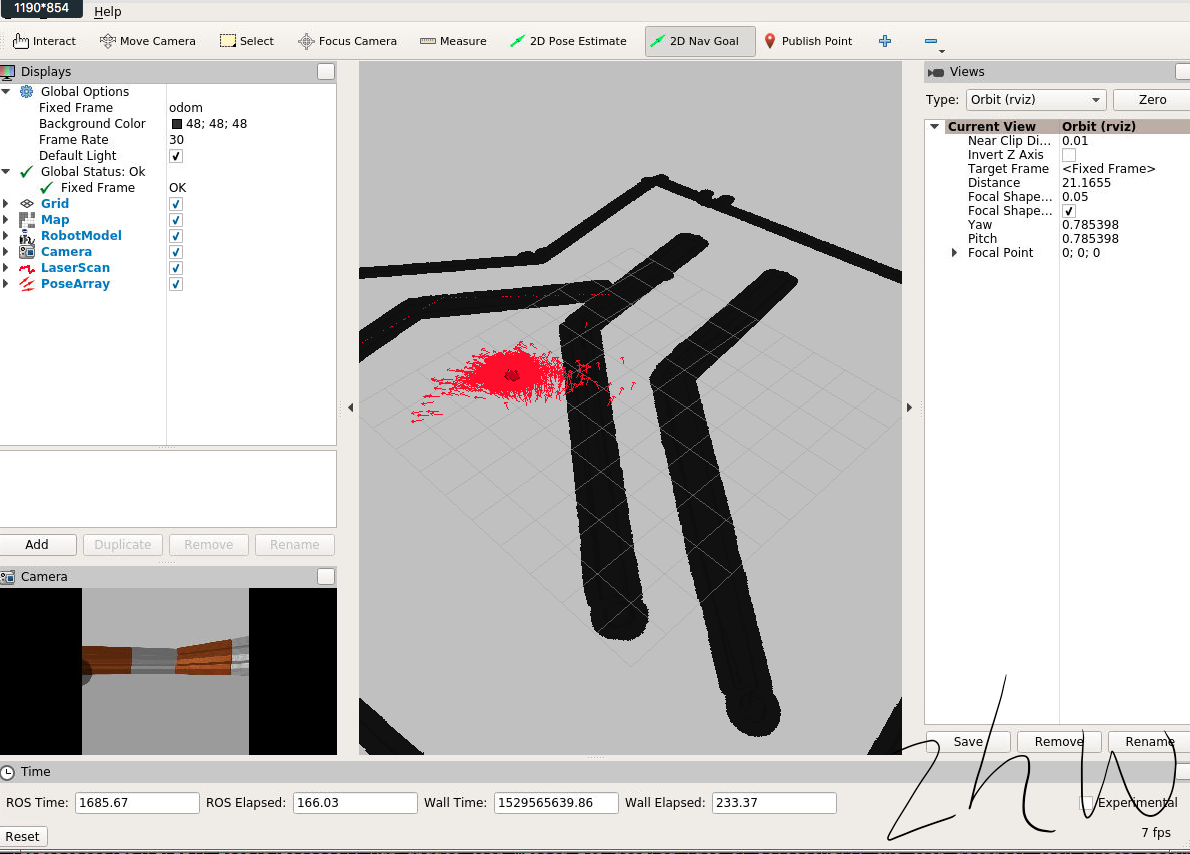
\includegraphics[width=0.5\textwidth]{r3.png}
\caption{\label{fig:result11}Result 1:Benchmark robot has reached the goal position and pass the test.}
\end{figure}

\begin{figure}
\centering
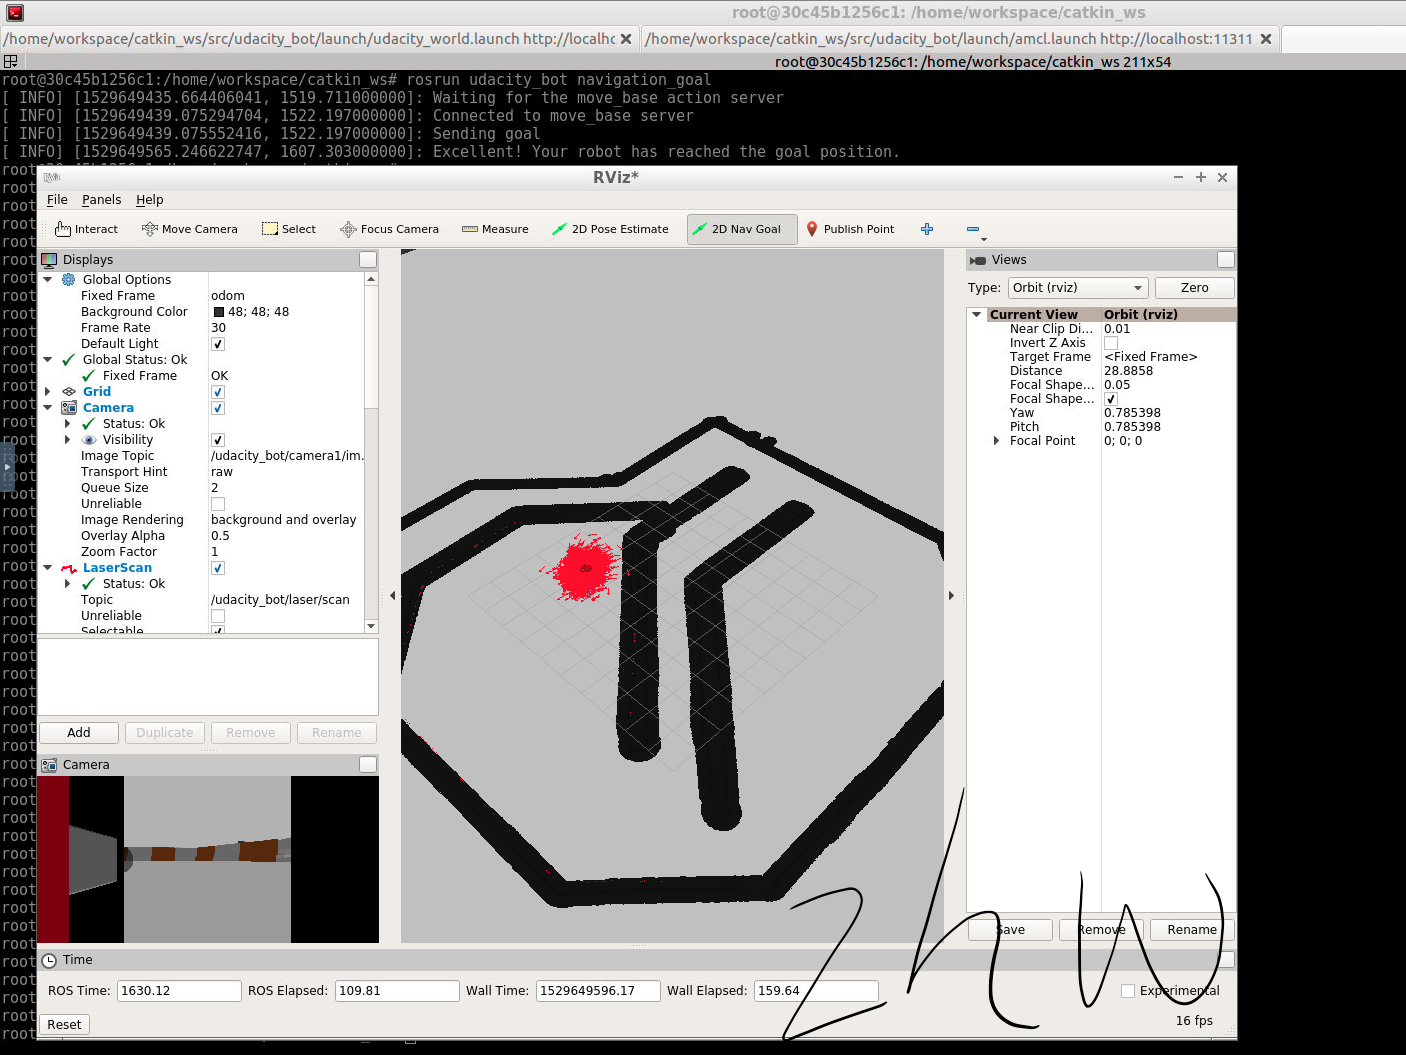
\includegraphics[width=0.5\textwidth]{r0.png}
\caption{\label{fig:result12}Result 1:Benchmark robot has reached the goal position and pass the test.}
\end{figure}

\subsubsection{Student}
See the Fig. \ref{fig:result2} 

\begin{figure}
\centering
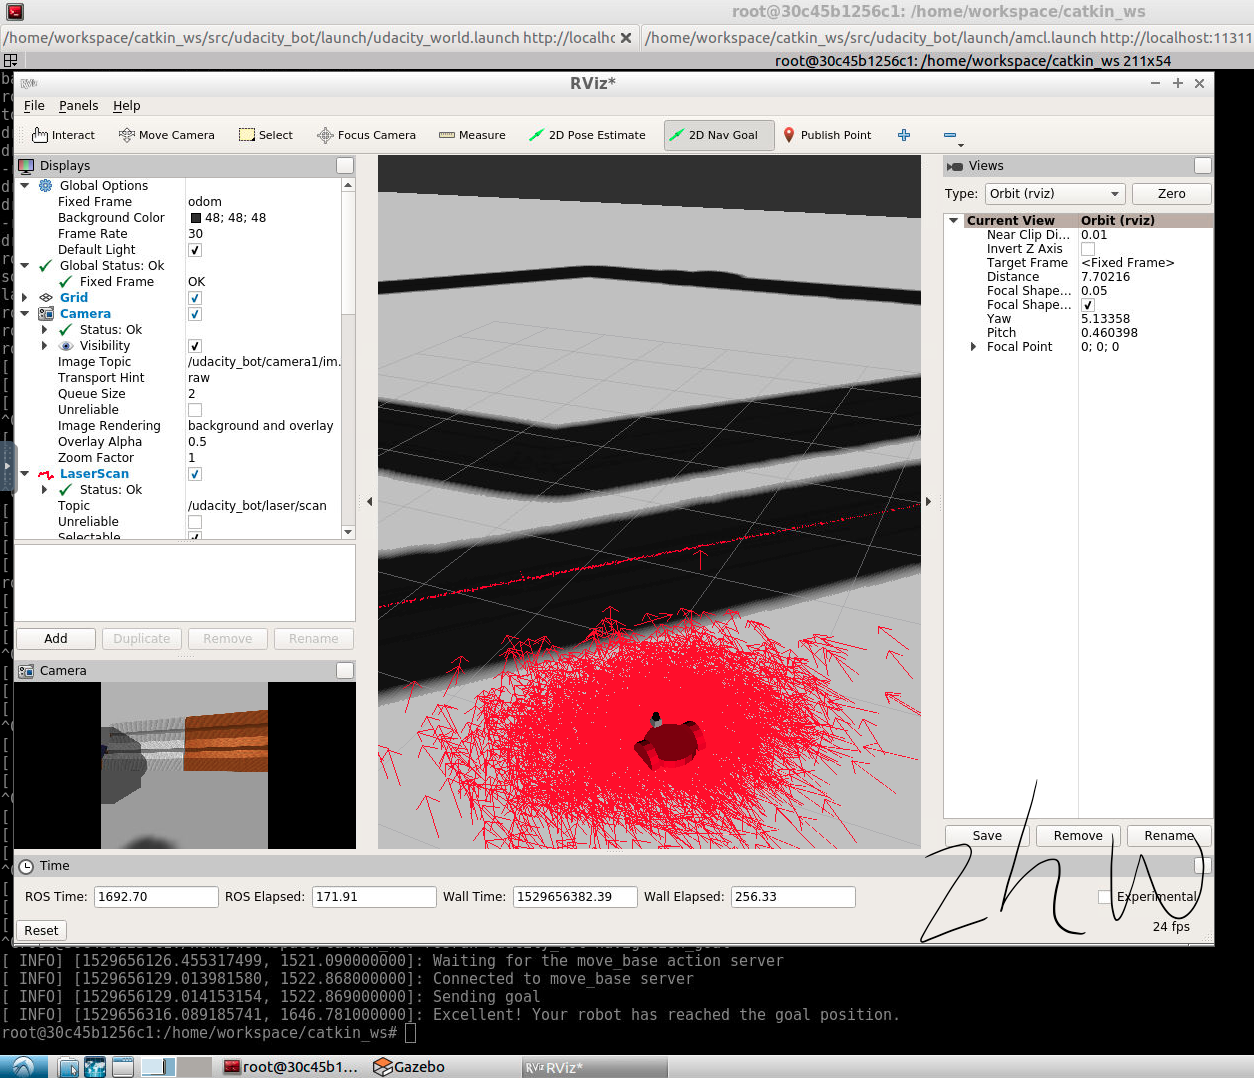
\includegraphics[width=0.5\textwidth]{r11.png}
\caption{\label{fig:result2}Result 2:Develop robot has reached the goal position and pass the test.}
\end{figure}



\subsection{Technical Comparison} 
At first, the parameters used in Benchmark robot is also used to run the own robot model, the performance are all worse than the Benchmark. But some of them are more flexible and faster. After a long time tuning parameters, when improve the inflation\_radius "0.3" to "0.6" and add parameters max\_vel\_x"0.4" and min\_vel\_x"0.1", it get a good result for the custom robot to reach the goal faster than the Benchmark robot. Inflation\_radius parameters help the robot get away from the obstacle and quickly find the 
best orientation. Parameters max\_vel\_x  and min\_vel\_x"0.1" help the robot to control the running speed and avoid hit the obstacle.

\section{Discussion}
There are many different develop models are test, in the project the develop robot performed better then the based model. The influences in conclusion, the control wheels size, the length between wheels, the position of the camera and Hokuyo and the stable of the chassis it's important to contribute the sensor layout and performance. The robot performed better with low center of gravity, smaller size of wheel size and a more stable chassis by adding four bottom wheel. And the shape of the chassis with circle in XY axis is greater than others to avoid hit the obstacle when change the orientation.

\section{Conclusion / Future work}

In the project, there are lots of work to utilize ROS packages to accurately localize a mobile robot inside a provided map in the Gazebo and RViz simulation environments. Building a good mobile robot is also a hard tasks for simulated and there are many more parameters in each package did not explore, with more parameters tuned the robot would achieve a better localization and perform result.


\subsection{Modifications for Improvement}

\begin{itemize}
\item Base Dimension 
\item Sensor Location
\item Sensor Layout
\item Sensor Amount
\item Center of gravity
\item Wheels size
\item Wheels Amount
\item chassis shape
\end{itemize}

\subsection{Hardware Deployment}
\begin{enumerate}
\item The Jetson TX2 board with ROS to explore. 
\item Computation time/resource improvement.
\item Add more sensor with sensor fusion 
\end{enumerate}


\bibliography{bib}
\bibliographystyle{ieeetr}

\end{document}